\section{Overview}
\label{sec:overview}

We are interested in the generation of test inputs comprised of
sequences of \emph{events} handled by the system-under-test (SUT); the
order of these events in the sequence is relevant to the property
being checked because of latent dependencies or effects they induce.
Examples of applications in which tests are naturally crafted in this
fashion include:
\begin{enumerate}

\item \textbf{Library API invocations:} The SUT is a library
  implementing an effectful abstract data type (ADT) with a set of
  APIs.  A test consists of a sequence of API calls that lead the
  implementation to an error state.

\item \textbf{Serialized input:} The SUT is a procedure that processes
  serialized input data, and reconstructs an AST from this input.  The
  inputs produced by the test generator are expected to establish
  semantic dependencies among nodes in the corresponding AST that do
  not satisfy a property of interest.

\item \textbf{Database transactions:} The SUT is a database supporting
  transactional read and write operations under various isolation
  levels.  A test consists of a sequence of transaction operations
  whose interleaved order is chosen to expose violations of isolation
  guarantees by the database.

\item \textbf{Distributed protocols:} The SUT is a distributed system
  whose components are expected to adhere to a protocol.  A test is a
  sequence of message invocations that lead the system to a global
  state in which protocol invariants are not maintained.
\end{enumerate}


%% SJ: belongs in intro.
%% A common feature shared by these examples, despite arising from
%% diverse domains, is that the test generator must be cognizant of how
%% event dependencies are (or are not) meaningful to manifesting a
%% property violation.  To do so, we define (1) a formal specification language
%% precisely describ latent dependencies
%% among operations; (2) a domain-specific language for expressing
%% generators that produce sequences conforming to these dependencies;
%% and (3) a program synthesis technique for automatically constructing
%% such generators from dependency specifications.

\subsection{Problem Setting}

More concretely, we consider how to apply our approach to the
well-studied~\cite{BeginnerLuck,CoverageType,FQL24} problem of testing
the correctness of an interpreter for simply-typed lambda calculus
(STLC) terms.  We focus on terms in which variables are represented by
their de Brujin index~\cite{DeBruijn} and seek to use PBT to discover
errors in an interpreter implementation that fails to correctly
increment the index during substitution under a lambda abstraction,
leading to incorrect variable capture.
\begin{align*}
  \text{\textsc{Reduction rule}:} \quad & (\lambda t. e)\; v \hookrightarrow e [0 \mapsto v]\\
  \text{\textsc{Incorrect substitution}:} \quad & (\lambda t. e)[n \mapsto v] = \lambda t. (e[\textcolor{red}{n} \mapsto v]) \quad \textcolor{red}{\xmark} \text{ \textcolor{gray}{should be $n + 1$}}
\end{align*}\noindent

Clearly, not all STLC terms have a structure whose reduction would
manifest this error.  In the following well-typed examples:
\begin{align*}
  \text{\textcolor{gray}{No bound variable:}} \quad & 2 \label{ex:e1}\tag{$e_1$}\\
  \text{\textcolor{gray}{Already in normal form:}} \quad & \lambda \Int. \lambda (\Int\sarr\Int).  ([0]\;[1]) \label{ex:e2}\tag{$e_2$}\\
  \text{\textcolor{gray}{Bound variable is not used:}} \quad & (\lambda (\Int\sarr\Int\sarr\Int). 3)\; (\lambda \Int. \lambda \Int. [1]) \label{ex:e3}\tag{$e_3$}\\
  % \text{\textcolor{gray}{Bound variable has index 0:}} \quad & (\lambda \Int. [0])\; 2 \tag{$\alpha_3$}\\
  \text{Term that triggers the bug:} \quad & (\lambda \Int. (\lambda (\Int\sarr\Int). [0]\;[1])\; (\lambda \Int. [0]))\; 3 \label{ex:e4}\tag{$e_4$}\\
  &\hookrightarrow (\lambda (\Int\sarr\Int). 3\;[1])\; (\lambda \Int. 3)  \quad \text{\textcolor{red}{wrong substitution}} \\
  &\hookrightarrow  3\;[1] \quad \text{\textcolor{red}{stuck!}}
\end{align*}\noindent
only \ref{ex:e4}'s evaluation involves an interesting use of
substitution and index manipulation.  Here, a buggy implementation
results in the argument value $3$ being mistakenly substituted for the
bound variable ``$[0]$'' in the two inner abstractions, instead of
``$[1]$''. In contrast, in $e_1$, $e_2$, and $e_3$,
the term is either already in normal form ($e_1$, $e_2$)
or performs a substitution that does not involve changing the value of
any index ($e_3$).

To expose this substitution bug, the generator should prioritize the
generation of terms similar to $e_4$ while avoiding those like
$e_1$--$e_3$.  To do this, it needs to at least adhere to
the following constraints:
\begin{enumerate}
  \item The test must contain at least one function abstraction (to rule out $e_1$).
  \item The test must be reducible, and not already in normal form (to rule out $e_2$).
  \item The body of every function abstraction must reference its
    bound variable (to rule out $e_3$).
\end{enumerate}
Although these constraints do not fully capture the intricate
dependencies required to generate test sequences like $e_4$ — and,
in practice, users may not know the exact conditions necessary to
expose such bugs in advance — they nonetheless significantly restrict
the search space of feasible terms and increase the probability of
uncovering the fault.

\begin{figure}[th!]
\begin{minted}[xleftmargin=5pt, numbersep=4pt, linenos = true,  escapeinside=??]{OCaml}
  type ty = Int | Arr of ty * ty
  type serialized_term = Const of int | Var of int | Abs of ty | EndAbs
                       | App | AppL | AppR
\end{minted}
\vspace*{-.1in}
\caption{STLC terms in a serialized form.}
\label{fig:stlc-syntax}
\vspace*{-.1in}
\end{figure}

To frame test generation for this problem in terms of event sequences
as mentioned above, we consider a setting in which the generator
outputs \emph{serialized} terms, rather than ASTs (see
\autoref{fig:stlc-syntax}), offloading the task of transforming the
flattened sequence of tokens it produces into an AST representation,
to the interpreter.

The definitions of constants and variables are standard, and variables
carry their de Bruijn index. However, the usual function abstraction
constructor ``$\Code{Abs\;\mykw{of}\;ty * term}$'' is now represented
by two operations, ``$\Code{Abs\;\mykw{of}\;ty}$'' and
``$\Code{EndAbs}$'', where the function body is the term that is
generated between them.  Similarly, the typical application constructor
``$\Code{App\;\mykw{of}\;term * term}$'' is now captured by three
operations: ``$\Code{App}$'', ``$\Code{AppL}$'', and ``$\Code{AppR}$''
that prefaces the application ($\Code{App}$), marks the beginning of
the argument ($\Code{Appl}$), and signals the end of the application
($\Code{AppR}$).

An example of a serialized STLC term is shown below, where we color
the corresponding parts of the term and the serialized term for better
readability.
\begin{align*}
  \text{\textcolor{gray}{STLC term:}} \quad & \textcolor{blue}{(\lambda \Int}. \textcolor{orange}{[0]} \textcolor{blue}{)}\; \textcolor{DeepGreen}{3} \\
  \text{\textcolor{gray}{serialized STLC term:}} \quad & \eff{app}; \textcolor{blue}{\zevent{abs}{\Int}}; \textcolor{orange}{\zevent{var}{0}}; \textcolor{blue}{\eff{endAbs}}; \eff{appL}; \textcolor{DeepGreen}{\zevent{const}{3}}; \eff{appR}
\end{align*}\noindent
We denote de Bruijn indices with ``$[...]$'' to distinguish them from
constants.  and write ``$\eff{op}(\emph{args})$'' to represent a constructor
application ``\Code{Op}(\emph{args})''
in a test sequence, for clarity.  The interpreter accepts a
serialized lambda term and evaluates it to a value. In the example
above, the input sequence should be reduced as $(\lambda \Int. [0])\;3
\hookrightarrow 3$.

To quantify the difficulty of having a testing framework produce terms
like \ref{ex:ex4}, we adapted a well-typed STLC
generator~\cite{BeginnerLuck,CoverageType} to output serialized terms
as described above, and tried to use it to find a substitution
violation in a known buggy interpreter that implements the incorrect
substitution rule described above.  It took 45 minutes and 275,915
attempts for the PBT system to find this bug.  This was because most
of the STLC terms that were generated were similar to
\ref{ex:e1}--\ref{ex:e3}, which do not use bound variables in an
interesting way.  The result is not particularly surprising given that
the baseline generator only knows how to generate well-typed terms,
and not well-typed terms intended to trigger a substitution error.
Adapting the generator to constrain the terms it generates as
described above requires additional context-sensitive tracking of
variable usage that is non-trivial to implement.  In the following, we
show how \tyName\ specifications can be used for this purpose to
synthesize such generators automatically.

\subsection{Temporal Trace Types, \tyName}

\paragraph{Traces and Trace-Based Specifications}
We refer to the sequence of events that comprise a test sequence as a
\emph{trace}. In our running example, traces consist of tokens drawn
from the grammar shown in \autoref{fig:stlc-syntax}.  Constraints
on these tokens can often be naturally expressed using temporal logic
or regular expressions. For example, the constraint that the term must
contain at least one abstraction can be expressed as a regular
expression (regex) $\allA \eff{abs} \allA$; here, $\allA$ denotes the
set of all traces, and $\eff{abs}$ represents the occurrence of a
function abstraction.  However, the third constraint, which requires
that \emph{for every} pair of an $\eff{abs}$ token and its
corresponding $\eff{endAbs}$ token, there exists a $\eff{var}$ event
within the body necessitates some form of universal quantification
over events. Similarly, a well-typedness constraint involves
establishing data dependencies and is naturally defined inductively
over the syntax of terms, making it challenging to express as a
uniform trace property that precisely distinguishes well-typed traces.

To address these concerns, we decompose global trace properties into
local specifications assigned as types to individual operations.  In
other words, we allow type-level specifications to be associated with
each event in a trace, enabling the specification of complex
constraints in a modular fashion, transferring the burden of event
quantification and data dependency management from a trace-level
specification language to the type system itself.  Concretely, we
model these local specifications as a collection of operation
signatures: parameter types constrain the payloads of events, while
the return type captures relationships between events. We employ
symbolic regular expressions (SREs) to qualify trace-based properties
within a type, following prior work on trace-based type
systems~\cite{KT+14,ZYDJ24,NUKT+18}. However, our formulation
generalizes beyond history-sensitive specifications of effects or
state, allowing types to express latent dependencies among all events,
including those that may occur in the future.

%% Thus, the return type of
%% an operation can include both a ``rely'' component, specifying
%% assumptions about prior events (the history regex) that allow this
%% type to be manifested, and a ``guarantee'' component (the prophecy
%% regex) that constrains future events.

\begin{figure}[t!]
  {\footnotesize
    \begin{align*}
      \eff{const} :~ &  x{:}\Int\sarr \rg{\allA}{\msgA{const}{x}}{\msgAGray{putType}{\CInt} \allA} \\
      \eff{app} :~ & \rg{\allA}{\msgC{app}}{\allA  \msgAGray{getType}{\Code{Arr}(t_1, t_2)}  \msgC{appL}  \allA  \msgAGray{getType}{t_1}  \msgC{appR}  \msgAGray{putType}{t_2}  \allA} \\
      \eff{abs} :~ & \rg{\allA\msgAGray{getDepth}{d}}{\msgA{abs}{t_2}}{\msgAGray{putDepth}{d+1}\allA  \msgC{var}  \allA  \msgAGray{getTy}{t_1}  \msgC{endAbs}\msgAGray{putDepth}{d}
        \msgAGray{putTy}{\Code{Arr}(t_1,t_2)}  \allA} \\
      \eff{var} :~ &  i{:}\ort{\Int}{\vnu \geq 0} \sarr \rg{\underbrace{\allA\msgA{abs}{t}\msgAGray{putDepth}{d}(\anyA\setminus\msgC{endAbs})^*}_\text{type $t$ at the $d$ level is open}\underbrace{\msgAGray{getDepth}{d + i}}_\text{current level is $d + i$} }{\msgA{var}{i}}{\msgAGray{putTy}{t}  \allA}
      % \eff{ascribe} :~ &  t{:}\Code{ty}\sarr \rg{\allA(\msgC{const} \lor \msgC{var} \lor \msgC{endAbs} \lor \msgC{appR} )}{\msgAGray{ascribe}{t}}{\allA} \\
      % \eff{depth} :~ &  t{:}\Code{ty}\sarr \rg{\allA(\msgC{const} \lor \msgC{var} \lor \msgC{endAbs} \lor \msgC{appR} )}{\msgAGray{ascribe}{t}}{\allA}
    \end{align*}
  }
\vspace*{-.2in}
  \caption{\tyName{} specifications of STLC operations. } %
  \label{fig:spec}
\vspace*{-.15in}
\end{figure}


\paragraph{History, current, and prophecy regex specifictions} 
A \tyName\ has the form
$\rg{H}{\msgB{op}{\overline{x}}{\phi}}{F}$, where the three components
describe the history, current, and future regex (resp.) that
establish the context for any trace containing the event
$\eff{op}$. Each signature reads: ``If an operation matching
$\msgB{op}{\overline{x}}{\phi}$ appears in a prefix trace matched by
the history regex $H$, then the suffix trace will be matched by the
prophecy regex $F$.'' Intuitively, future regexes are a trace-based
analogue of prophecy variables~\cite{LM22} used in other state-based
concurrency reasoning approaches to constrain future events.

The \tyName\ specifications of the STLC operators in our motivating
example are shown in \autoref{fig:spec}.  The specifications consist
of two kinds of events.  \emph{Effect} events, given in
\textbf{bold}, and their ordering in a \tyName\ constrains
the shape of well-typed terms.  \emph{Ghost} events, depicted in
\textcolor{gray}{gray}, establish semantic dependencies in traces that
characterize notions of well-typedness and de Brujin index
representations in terms.  These events do not appear in synthesized
test generator programs.

\SJ{Stop here ...}

The type for $\eff{const}$ has no constraint on its prefix trace
($\allA$), but records a $\textcolor{gray}{\eff{putType}}$ event in
the trace that records the type of the output of the $\eff{const}$
expression as $\Code{Int}$.  The arguments to a ghost event are either
serialized terms (like $\Code{Int}$) or ghost variables.
Type-checking a trace using ghost events involves solving constraints
over their arguments based on algebraic axiomatizations, examples of
which are given below.  The prophecy regex of the $\eff{app}$ type in
\autoref{fig:spec} characterizes both the syntax and well-typing
constraints of an STLC function application. It requires that (a)
prior to evaluating a function argument ($\eff{appL}$), the type of
the abstraction is \Code{Arr(t$_1$,t$_2$)}, i.e., the abstraction
being applied is a function type ($\msgAGray{getType}{\Code{Arr}(t_1,t_2)}$), (b) after the argument is evaluated, its type is
  determined to be \Code{t$_1$} ($\msgAGray{getType}{t_1}$), and (c)
  the type of the application's result is \Code{t$_2$}
  ($\msgAGray{getType}{t_2}$).  
\footnote{The ghost variables
  (e.g., $t_1$ and $t_2$) are implicitly quantified at the top level,
  following the OCaml syntax convention. The event specifications
  $\msgA{op}{\overline{v}}$ and $\eff{op}$ are syntactic sugar for
  $\msgB{op}{\overline{x}}{\overline{x = v}}$ and
  $\msgB{op}{\overline{x}}{\top}$.}  Besides the atoms of the grammar,
types can include two additional events, $\eff{\textcolor{gray}{put}}$
and $\eff{\textcolor{gray}{get}}$ used to manage stateful properties
of a trace.

the postfix should contain two sub-terms separated by
$\eff{appL}$ and $\eff{appR}$ events, where the first and second
sub-terms are required to have type $t_1\sarr t_2$ and $t_1$ via
$\eff{\textcolor{gray}{getTy}}$ respectively, and then updated the
type of constructed term as $t_2$.

The type
of $\eff{app}$ captures
both the syntax and well-typing constraints of an application.
It imposes no constraints on the event sequence in its history,
but requires that the future trace should contain two arbitrary
subterms (denoted by $\allA$), separated by
$\eff{appL}$ and $\eff{appR}$ events.   The value of
$\Code{ttype}$ in the first subterm is $\Code{Arr(t_1,t_2)}$,
where $\Code{t_1}$ and $\Code{t_2}$ are elements of $\Code{ty}$,

sub-terms are required to have type $t_1\sarr t_2$ and $t_1$ via
$\eff{\textcolor{gray}{getTy}}$ respectively, and then updated the
type of constructed term as $t_2$.


In
order to help specify the implicit state of test sequence generation,
we add auxiliary $\eff{\textcolor{gray}{put}}$ and
$\eff{\textcolor{gray}{get}}$ operator for the type and depth of
nested function abstractions of current contructed term. These
operators can also help to synthesize statful test generators.  For
example, the first type in \autoref{fig:spec} characterizes the
behavior of $\eff{const}$ messages. It has no constraint on its prefix
trace ($\allA$), but requires that the postfix trace first update the
type of current constructed term as $\Int$.

The de Bruijn index constraint is captured via the $\eff{\textcolor{gray}{putDepth}}$ and $\eff{\textcolor{gray}{getDepth}}$ operation in the \PAT{}s of the $\eff{abs}$ and $\eff{var}$ operations. In addition to the well-typing constraint, the \PAT{} of the $\eff{abs}$ operation maintains the depth of nested function abstractions using $\eff{\textcolor{gray}{depth}}$. Specifically, its history regex obtains the current depth ($\msgAGray{getDepth}{d}$), increases it by one at the beginning of the function body, and restores it after the $\eff{endAbs}$ event. Moreover, its prophecy regex also uses a $\eff{var}$ event to require that the body of the function abstraction references its bound variable at least once, thereby ruling out terms like $e_1$.
On the other hand, a valid index $i$ in $\eff{var}$ must be derived from an open abstraction at some depth in the prefix trace. The history regex of the $\eff{var}$ operation precisely characterizes this constraint: the abstraction at depth $d$ must be open ($\allA\msgA{abs}{t}\msgAGray{putDepth}{d}(\anyA\setminus\msgC{endAbs})^*$), and the current depth must be $d + i$.

The \PAT{}s shown in \autoref{fig:spec} demonstrate that \PAT{}s are powerful enough to specify the de Bruijn index constraint and well-typedness of STLC in a compact manner. These relations capture scoping, indexing, and non-trivial recursive typing relationships. With help of these \PAT{}s, we can define a global property that exactly captures the three constraints that rule out \ref{ex:e1}--\ref{ex:e3} as the following:
\begin{align*}
  \msgAGray{putDepth}{0}\allA \eff{abs} \allA \msgAGray{getTy}{\Int} \label{prop:stlc}\tag{$A_\Code{STLC}$}
\end{align*}\noindent
where we first specify the initial depth as 0 and required the final constructed term to be a well-typed term of type $\Int$.

% Its history
% regex describes how a $\eff{writeReq}$ message is handled in an
% arbitrary context ($\allTL$, where $\globalA$ is the globally modality
% in LTL$_f$), and its prophecy regex guarantees that a
% $\eff{writeRsp}$ response message will eventually be issued at some
% future point, as captured by the $\finalA$ operator.  This
% specification captures the asynchronous behavior of request/response
% pairs in our example, requiring that the handler of $\eff{writeReq}$
% eventually triggers a $\eff{writeRsp}$ message. On the other hand, we
% assume little information about the behaviors of the handlers for
% $\eff{readRsp}$ and $\eff{writeRsp}$ messages, as can been seen by
% their prophecy regex, which provide no guarantees about any future
% messages they may produce ($\allTL$).

% \paragraph{Control flow} A handler's \PAT{} also captures  relevant
% control-flow dependencies. For example, the type of $\eff{readReq}$
% uses an intersection type ($\interty$) to encode its behaviors in the
% two different contexts under which a $\eff{readReq}$ message may be
% handled, corresponding to whether or not some value has been
% previously written to the database. The first \PAT{} specifies that
% the handler must eventually respond with the last value that was
% requested to be written, as captured by the history regex: %
% {
%   $ \finalA \msg{writeReq}{v = \Code{x}} \land
%   \neg\nextA\finalA\msg{writeReq}{\top} $ } %
% and prophecy regex %
% { $\msg{readRsp}{v = \Code{x} \land st = \true}$ }.
% Otherwise, as specified by the second \PAT{}, no value has been
% successfully written ($\neg\finalA \msg{writeRsp}{\top}$), and a
% $\eff{readRsp}$ message with a $\false$ status will eventually be sent
% ($\finalA\msg{readRsp}{st = \false}$).

% This specification is sufficiently weak to allow a controller to probe
% for violations of the RYW property.  Specifically, $\eff{readReq}$'s
% specification allows a successful $\eff{readRsp}$ to return the value
% in the database that exists at the time the $\eff{readReq}$ message is
% handled, ignoring the possibility of other $\eff{writeRsp}$ messages
% that are executed after the $\eff{readReq}$ but before the
% corresponding response.  This is precisely the scenario depicted by
% the controller program $P_C$ in \autoref{fig:2pc-term} (lines 5-7).
% On the other hand, a stronger specification for $\eff{writeReq}$ would
% restrict the controller to focus on executions that exhibit write
% atomicity, e.g., prohibiting a $\eff{readReq}$ operation from being
% handled before a $\eff{writeRsp}$, thus preventing executions that
% would manifest a RYW violation:

% {\footnotesize
%   \begin{align*}
%     \mykw{gen}~ \eff{writeReq} :~ &  \Code{x}\hasnty{int} \sarr \rg{\allTL}{\msg{writeReq}{v = \Code{x}}}{(\neg \msg{readReq}{\top}) \untilA \msg{writeRsp}{v = \Code{x}}}
%   \end{align*}}\noindent
% \PAT{}s thus provide an expressive framework in which to specify the
% set of executions that are of interest to the test engineer, grounded
% in the semantic relationships that are expected to hold among
% different actors in the model: weaker specifications admit more
% behaviors, at the potential cost of trying to explore executions that
% are not realizable by the actors' implementations; stronger specifications
% restrict this set, at the cost of excluding some potentially erroneous executions.

\subsection{DSL}

\newcommand{\ranint}{\underline{\Code{int\_gen\;()}}}

\begin{figure}
\centering
\begin{minted}[xleftmargin=5pt, numbersep=4pt, linenos = true, fontsize = \footnotesize, escapeinside=??]{OCaml}
let rec lam_body_gen (n: int) =
  (?$\eff{var}$? n) ?$\oplus$? // ?$\textcolor{DeepGreen}{[n]}$?
  (?$\eff{app}$?;
     ?$\eff{abs}\;\Int\sarr\Int$?; ?$\eff{app}$?; ?$\eff{var}$? 0; ?$\mykw{obs}\;\eff{appL}$?; lam_body_gen (n+1); ?$\mykw{obs}\;\eff{appR}$?; ?$\mykw{obs}\;\eff{endAbs}$?;
     // ?$\textcolor{DeepGreen}{\lambda (\Int\sarr\Int). ([0]\;(\underline{\Code{lam\_body\_gen}\;(n + 1)}))}$?
   ?$\mykw{obs}\;\eff{appL}$?; ?$\eff{abs}$? int; ?$\eff{var}$? 0; ?$\mykw{obs}\;\eff{endAbs}$?; // ?$\textcolor{DeepGreen}{\lambda \Int. [0]}$?
   ?$\mykw{obs}\;\eff{appR}$?) // ?$\textcolor{DeepGreen}{\lambda (\Int\sarr\Int). ([0]\;(\underline{\Code{lam\_body\_gen}\;(n + 1)}))\;\lambda \Int. [0]}$?
in
?$\eff{app}$?; ?$\eff{abs}$? int;f 0; ?$\mykw{obs}\;\eff{endAbs}$?; // ?$\textcolor{DeepGreen}{\lambda \Int. (\underline{\Code{lam\_body\_gen}\;0})}$?
?$\mykw{obs}\;\eff{appL}$?; ?$\eff{const}$? (int_gen ()); // ?$\textcolor{DeepGreen}{\ranint}$?
?$\mykw{obs}\;\eff{appR}$?; // ?$\textcolor{DeepGreen}{\lambda \Int. (\underline{\Code{lam\_body\_gen}\;0})\;(\ranint)}$?
\end{minted}
\vspace*{-.1in}
\caption{STLC generator $P_\Code{STLC}$. }\label{fig:stlc-gen}
\vspace*{-.2in}
\end{figure}

With \PAT{}s of operators and global property \ref{prop:stlc}, our tool can synthesize a test generator $P_\Code{STLC}$ in our DSL shown in \autoref{fig:stlc-gen} where we omit all auxiliary operations for simplicity. Our DSL is mostly similar with standard OCaml program with the STLC operations as function application ($\eff{op}$ and $\mykw{obs}\;\eff{op}$). This generator produce terms in a form ``$\lambda \Int. (\underline{\Code{lam\_body\_gen}\;0})\;(\ranint)$'' (line 9 - 11), where $\Code{lam\_body\_gen}$ (line 1 - 7) is a recurisve function that has two branches concatenated with a non-deterministic choice ($\oplus$) on line 2. The first branch returns a bound variable always refers the $\ranint$ and has index $n$ which is equal to the current depth of nested function abstractions. The second branch (line 3 - 7) returns a STLC term in the form $\lambda (\Int\sarr\Int). ([0]\;(\underline{\Code{lam\_body\_gen}\;(n + 1)}))\;\lambda \Int. [0]$. The generator will non-deterministically unfold the recursive function and produce the following STLC terms:
\begin{align*}
  \text{1 iteration:} \quad & (\lambda \Int.\textcolor{blue}{[0]})\;3 \\
  \text{2 iterations:} \quad & (\lambda \Int. \textcolor{purple}{(\lambda (\Int\sarr\Int). [0]\;\textcolor{blue}{[1]})\; (\lambda \Int. [0])})\; 3 \tag{exactly \ref{ex:e2}}
  \\
  \text{3 iterations:} \quad & (\lambda \Int.\textcolor{pink}{(\lambda (\Int\sarr\Int). [0]\;\textcolor{purple}{(\lambda (\Int\sarr\Int). [0]\;\textcolor{blue}{[2]})\; (\lambda \Int. [0])})\; (\lambda \Int. [0])})\; 3
\end{align*}\noindent
The term generated by 2 or more iterations can trigger the substitution bug in the interpreter.

\paragraph{Generative and derived terms}
The STLC operations are distinguished as either generative or derived operations ($\mykw{obs}$), where the former can be generated without constraint, but the latter must be derived from other operations. For example, the $\eff{endAbs}$ operation is derived from the generative $\eff{abs}$ operation; the $\eff{appL}$ and $\eff{appR}$ operations are derived from the generative $\eff{app}$ operation. Our DSL ensures the pairing relationship between generative and derived operations, which guarantees that the generated trace is well-formed with respect to STLC syntax. This feature is also crucial for test generators in other domains—for example, the pairing of $\eff{init}$ and $\eff{close}$ in the effectful library, the scoping relationship of $\eff{begin}$ and $\eff{commit}$ transactions in databases, and the correspondence between request and response messages in distributed systems.

\paragraph{Typechecking} Specifying the behavior of operations in terms of
\PAT{}s allows us to use a type system to statically check that
test generator programs will only generate the expected traces.
For example, to typecheck the use of $\eff{app}$ on line 9 in
\autoref{fig:stlc-gen}, we first ``divide'' the generator $P_\Code{STLC}$ into three pieces:
an empty history subprogram, a current event ($\eff{app}$), and a future subprogram on lines 9--11. The first subprogram corresponds to the set of prefix traces that can occur before
$\eff{app}$, while the last subprogram captures all the postfix traces that may follow.
Thus, we must ensure that each of these pieces
is consistent with the type of $\eff{app}$, which requires correct scoping and well-typedness of STLC terms.
Note that the future subprogram contains $\eff{appL}$ (line 10) and $\eff{appR}$ (line 12) operations, which are derived from the generative $\eff{app}$ operation. The term between $\eff{appL}$ and $\eff{appR}$ is a lambda abstraction with type $\Int\sarr\Int$, and the term between $\eff{app}$ and $\eff{appL}$ is a constant with type $\Int$. Checking the type of $\eff{abs}$ on line 9 is more intriguing, as its prophecy regex requires at least one $\eff{var}$ usage in the body of the function abstraction. This constraint is satisfied on line 2—no matter how many times the recursive function is unfolded, it always returns on line 2 and uses the bound variable at least once. Our type system can also check that the generator $P_\Code{STLC}$ is consistent with the global specification \ref{prop:stlc}, which requires that the generated STLC term has type $\Int$ and contains at least one lambda abstraction (line 9).


% that
% the last value written to the database is $\Code{y}$ (line $3$) in the
% history, that the message being handled is $\eff{readReq}$, and that a
% $\eff{readReq}$ message with value $\Code{y}$ will be produced in the
% future (line $7$). Notably, $P_{C}$ can indeed induce a trace that
% violates RYW consistency. We can show this by typechecking $P_{C}$
% against the \PAT{} $\rg{\epsTL}{\negSCA}{\epsTL}$. This \PAT{} asserts
% that when there are no prior messages ($\epsTL$), the execution of the
% controller generates a trace consistent with \ref{eqn:autoEx}, and no
% more future messages are generated ($\epsTL$).

\subsection{Test Generator Synthesis}

\begin{figure}[ht!]
\vspace*{-.15in}
    \centering
    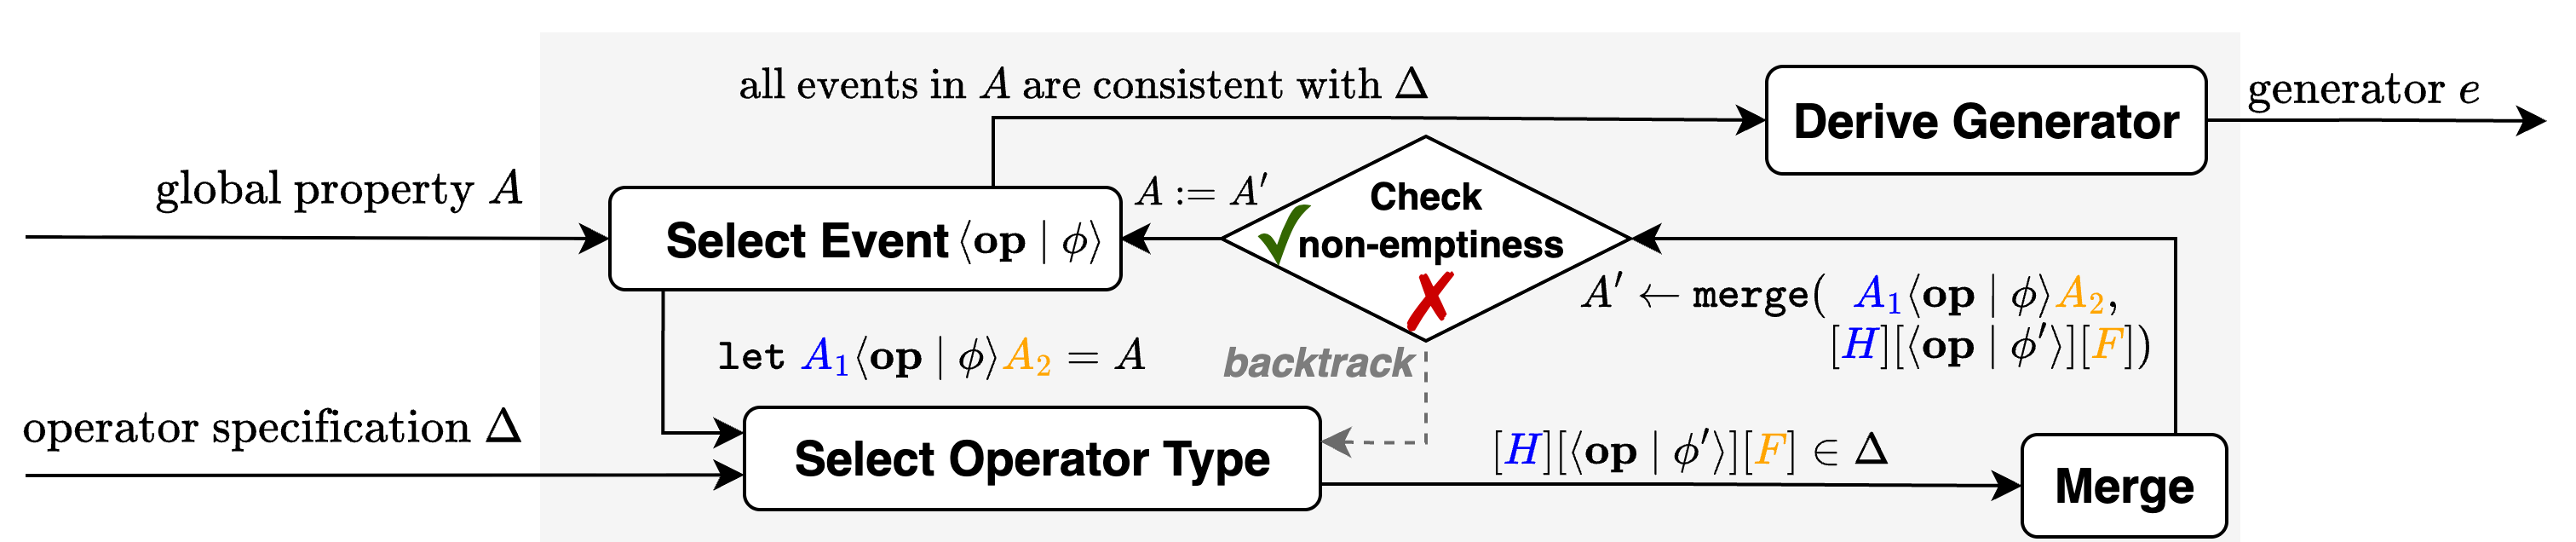
\includegraphics[width=1.0\linewidth]{figures/pret.drawio.png}
\vspace*{-.2in}
    \caption{Test controller synthesis pipeline.}
    \label{fig:intuition-algo}
% \vspace*{-.1in}
\end{figure}

Interpreting test sequences as traces allows us to frame the derivation of
a test generator as a component-based synthesis problem, guided by the
\PAT{} specifications of the operators (e.g., $\Delta$) and the global property (e.g., \ref{prop:stlc}). \autoref{fig:intuition-algo} provides a high-level overview of our
algorithm, which consists of two phases. In the first phase, we
systematically refine the global property $A$ to remove undesired test sequences (e.g., \ref{ex:e1}--\ref{ex:e3}). The resulting regex $A'$ encodes a stronger
property on traces, i.e., $A' \subseteq A$, ensuring that each
operation in the test sequence is consistent with its specification. In the second phase, we
use $A'$ to derive a test generator program. For example, the set of
traces captured by $P_\Code{STLC}$ can be refined from \ref{prop:stlc} to: %
\vspace{-.4cm} \par\nobreak
{\footnotesize
  \begin{align*}
  \msgAGray{putDepth}{0}\underbrace{\msgC{app}}_{\allA}&\msgA{abs}{\Int}\underbrace{...\msgC{endAbs}...\msgC{appL}\msgA{const}{\top}\msgAGray{putTy}{\Int}\msgAGray{getTy}{\Int}\msgC{appR}\msgAGray{putTy}{\Int}}_{\allA}\msgAGray{getTy}{\Int}
  \label{prop:refinedSTLC}\tag{$A_\Code{STLC}'$}
  \end{align*}}\noindent
This regex specializes the two Kleene stars in \ref{prop:stlc} as two sub-regexes as shown above. Note that from the view of each event, the corresponding prefix trace and postfix trace are aligned with its \PAT{}.
Observe that the structure of \ref{prop:refinedSTLC} closely resembles the
test generator program $P_\Code{STLC}$, with the main difference being that
$P_\Code{STLC}$ is more operational, dividing operations into generative and derived operations.

% The test generator also provides the contents for generative operations, while the contents of
% derived operations are constrained only by local variables.


\paragraph{Property Refinement Loop}
The refinement loop is a crucial piece of the algorithm in
\autoref{fig:intuition-algo}, as it ensures that the traces accepted
by the refined formula are consistent with our expectations of \PAT{}s. Viewed from another perspective, this algorithm searches
for a family of traces that witness a property violation until it finds one
that aligns with the provided specifications.
A key challenge is dealing with latent dependencies among events, where these events may be hidden under a Kleene star. For example, \ref{prop:stlc}
includes over 10 events, but only three of them appear in \ref{prop:refinedSTLC}
(i.e., $\eff{\textcolor{gray}{putDepth}}$, $\eff{abs}$, and $\eff{\textcolor{gray}{getTy}}$). While \PAT{}s allow us to add dependent events of one event into the global property, each of these new events can
impose additional requirements that must be satisfied. Naively inlining the \PAT{}s into the global property can easily cause the search space to grow exponentially.
To address this
challenge, our algorithm lazily injects new events into the test generator program, and then recursively repairs any unmet obligations. This allow our algorithm to smart event discover in both forward and backward directions.
As an example, when working on an top-level event (i.e., not under Kleene star) $\eff{abs}$, the algorithm aligns the \PAT{} of $\eff{abs}$ with the current formula and merges them as the following:
{\small\begin{align*}
  \underbrace{\msgAGray{putDepth}{0}\allA\msgAGray{getDepth}{0}}_\texttt{merged with history regex}\;\; \msgA{abs}{t_2}\;\; \underbrace{... \msgC{var} ... \msgC{endAbs}\msgAGray{putDepth}{d} \msgAGray{putTy}{t_1\sarr t_2}  \allA \msgAGray{getTy}{\Int}}_\texttt{merged with prophecy regex}
\end{align*}}\noindent
The updated formula clearly shows that the $\eff{abs}$ event imposes a requirement that multiple events happen before and after it, which will be marked as \PAT{}s that still need to be satisfied. Most interestingly, this procedure can be preformed backwardly, which allows our algorithm to discover the previous event who triggers the unsolving event. For example, when working on the last $\eff{getTy}$ event, the algorithm identifies that it requires a previous $\eff{putTy}$ event to update the type of current constructed term as $\Int$, since the type of the lambda abstraction is a function type ($\msgAGray{putTy}{t_1\sarr t_2}$). Thus, the algorithm refines the current formula as the following:
\vspace{-.4cm} \par\nobreak {\small %
  \begin{align*}
   ... \msgC{endAbs}\msgAGray{putDepth}{d} \msgAGray{putTy}{t_1\sarr t_2}  \allA \underbrace{\msgAGray{putTy}{\Int}}_\texttt{new event discovered backwardly}  \allA \msgAGray{getTy}{\Int}
\end{align*}}\noindent
which guides the algorithm to discover other STLC constructor (e.g., $\eff{app}$) that can generate $\msgAGray{putTy}{\Int}$ events.

\paragraph{Recursion} After all top-level events are refined, the algorithm treats the remaining Kleene star as a placeholder for recursion. We adapt a standard template-based approach to generate simple recursions. For example, the recursion in $P_\Code{STLC}$ is derived from a recursive function template with an increasing index parameter. This approach is efficient for handling cases in PBT across different domains, including recursion for balanced $\eff{push}$ and $\eff{pop}$ and retry loops for system initialization.


% As an
% example, when working on a $\eff{\textcolor{gray}{ascribe}}$ message, the algorithm identifies that it is dependent with one of STLC constructor, i.e., $\eff{const}$, $\eff{var}$. Moreover, $\eff{readReq}$'s type
% also indicates that its content $\Code{y}$ should belong to a previous
% $\eff{writeReq}$.  Based on these constraints, our algorithm refines
% the current formula by adding $\eff{writeReq}$ and $\eff{readReq}$
% messages before $\eff{readRsp}$, and marks both as messages whose
% constraints still need to be satisfied as synthesis proceeds.
